\section{Calibration}

\subsection{Calibration algorithm}
\subsection{Calibration plots}

Since the SVT modules are designed with a binary readout system, the analog channel response cannot be measured directly. Instead, the analog response is reconstructed by injecting a calibration charge on the channel and measuring the corresponding occupancy over a range of threshold values. Noise is measured using external, low frequency calibration charge injected in the absence of signal. The injected charge is shaped and amplified in the analog circuitry to form an output signal. The discriminator threshold determines whether or not the output signal corresponded to a hit. The probability that the injected charge produces a hit depends on the setting of the discriminator threshold. The average hit probability is measured by repeating the process of injecting charges and counting the fraction of readout triggers that produced a hit. This measurement is repeated over a range of threshold settings to produce an occupancy plot. 

\begin{figure}[hbt] 
	\centering 
	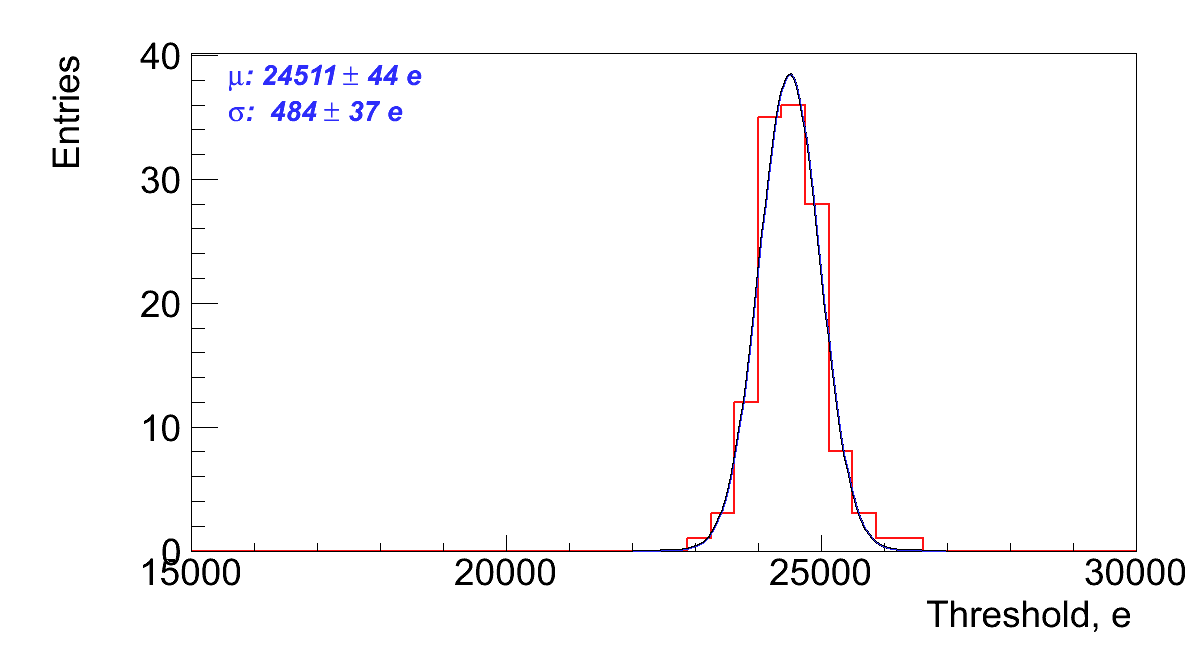
\includegraphics[width=0.5\columnwidth,keepaspectratio]{thrdisp.png}
	\caption{Typical threshold dispersion within a chip.}
	\label{fig:thrdisp}
\end{figure}

The occupancy plots were measured setting the pulser amplitude at fixed values and changing the comparator thresholds. Each point of an occupancy plot represents the percentage of times that the comparator fires for a certain value of injected charge. In between the high and low threshold regions, the occupancy curve is described by an error function, or S-curve, which can be fitted to the occupancy histogram for each channel, producing a mean value (discriminator threshold) and standard deviation (noise). The conversion from mV to electrons is performed considering a nominal value for the FSSR2 injection capacitance of 40~fF. 

\begin{figure}[hbt] 
	\centering 
	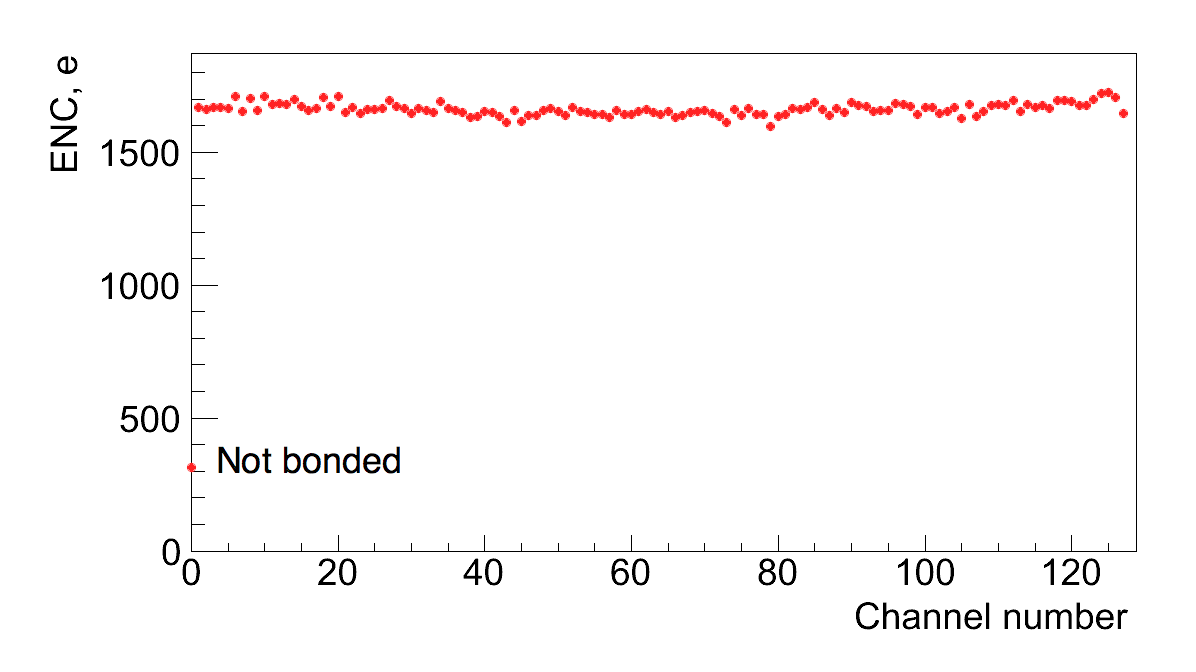
\includegraphics[width=0.5\columnwidth,keepaspectratio]{encmodule.png}
	\caption{Typical input noise on a single chip of an SVT module.}
	\label{fig:encmodule}
\end{figure}

Threshold dispersion is defined to be a standard deviation of the distribution of means obtained from the parameters of the complementary error function fit. The noise and threshold dispersion constants for each individual detector channel are measured and the values are used by the zero-suppression algorithms implemented in the core logic of the FSSR2 and by calibration procedures to identify defective channels. A comparison of the noise for 33~cm strips with the threshold spread demonstrates that the threshold spread is negligible compared to noise and does not affect efficiency and noise occupancy (see Fig.~\ref{fig:thrdisp}).

\section{Results of the Full Chain Test}

No significant correlated noise has been observed between the channels of the same chip, chips of the same module or closely placed modules. Measured average channel noise (see Fig.~\ref{fig:encmodule}) is comparable with estimated contributions of different noise sources. 

\begin{figure}[hbt] 
	\centering 
	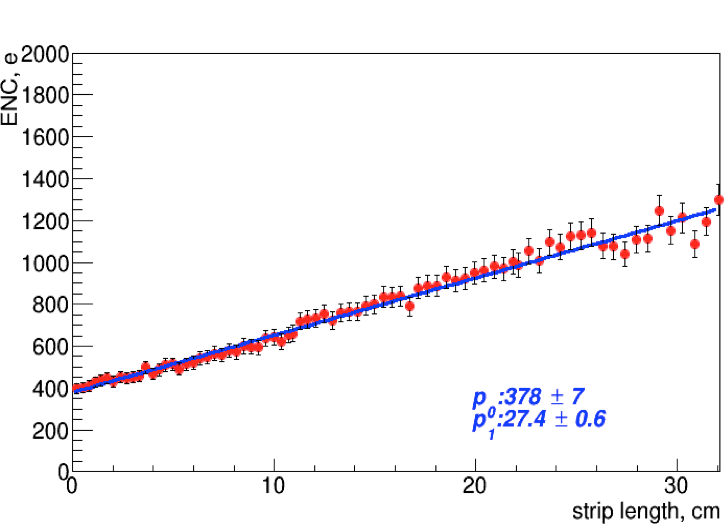
\includegraphics[width=0.5\columnwidth,keepaspectratio]{encstriplength.png}
	\caption{Input noise vs. strip length.}
	\label{fig:encstriplength}
\end{figure}

Longer silicon strips have higher capacitance and thus a higher input noise (see Fig.~\ref{fig:encstriplength}). Noise calibration accounts for the different strip lengths and pitch adapter layouts that affect the input capacitance of the preamplifier. The mean noise values scale linearly with strip length which confirms that the noise is dominated by the strip capacitance and not by coherent noise pickup of the system. 

Noise occupancy histogram with no charge injection is shown in Fig.~\ref{fig:noiseocc}. It probes the tail of the noise distribution, which can show effects masked by the higher occupancy at low thresholds. Channel noise allows setting a 3~$\sigma$ threshold at 30~keV level. 

\begin{figure}[hbt] 
\centering 
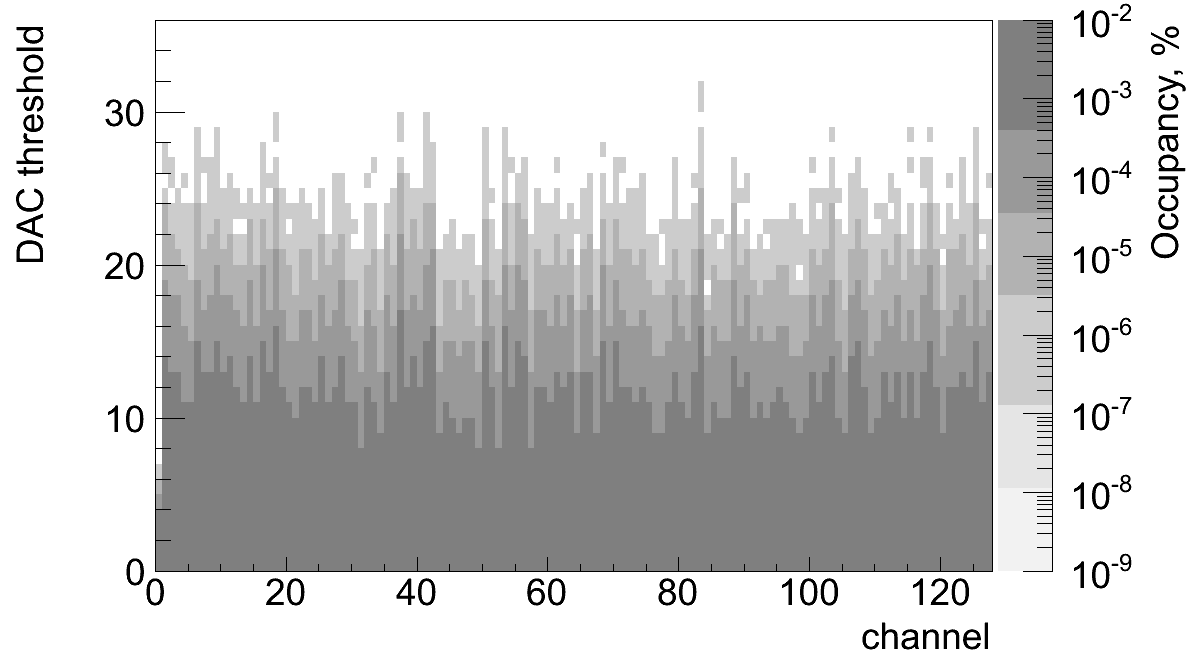
\includegraphics[width=0.5\columnwidth,keepaspectratio]{occ_thr.png}
\caption{Channel noise occupancy vs. DAC hit/no-hit threshold (in DAC bins, one DAC bin corresponds to 3.5~mV).}
\label{fig:noiseocc}
\end{figure}

Detector performance was tested by calibration procedures. Noise calibration accounts for the different strip lengths and pitch adapter layouts that affect the input capacitance of the preamplifier. Channel noise has linear dependence on the strip length from 400 electrons for the shortest strips. Defects known before the integration of the system were reestablished. 99.9$\%$ of channels are operational after detector integration. Noise behavior is found to be very good and well understood. No significant correlated noise has been observed between the channels of the same chip, between the chips of the same module or between the closely placed modules. 

\begin{figure}[hbt] 
	\centering 
	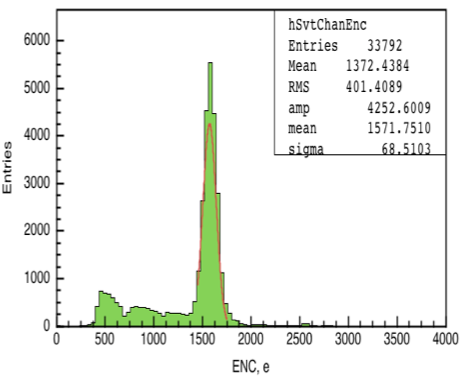
\includegraphics[width=0.5\columnwidth,keepaspectratio]{enc.png}
	\caption{SVT channel noise.}
	\label{fig:enc}
\end{figure}

Equivalent Noise Charge (ENC) of the SVT channels is shown in  Fig.~\ref{fig:enc}. The peak is $\sim$1600 electrons, the shoulder on the left side corresponds to the shorter strips. Channel noise allows setting a 3$\sigma$ threshold at 20~keV level. Noise is found to be stable and the the dependence of the noise on the environmental temperature and humidity is small. Noise performance in the experimental hall was comparable with results taken in the clean room. 

\begin{figure}[hbt] 
	\centering 
	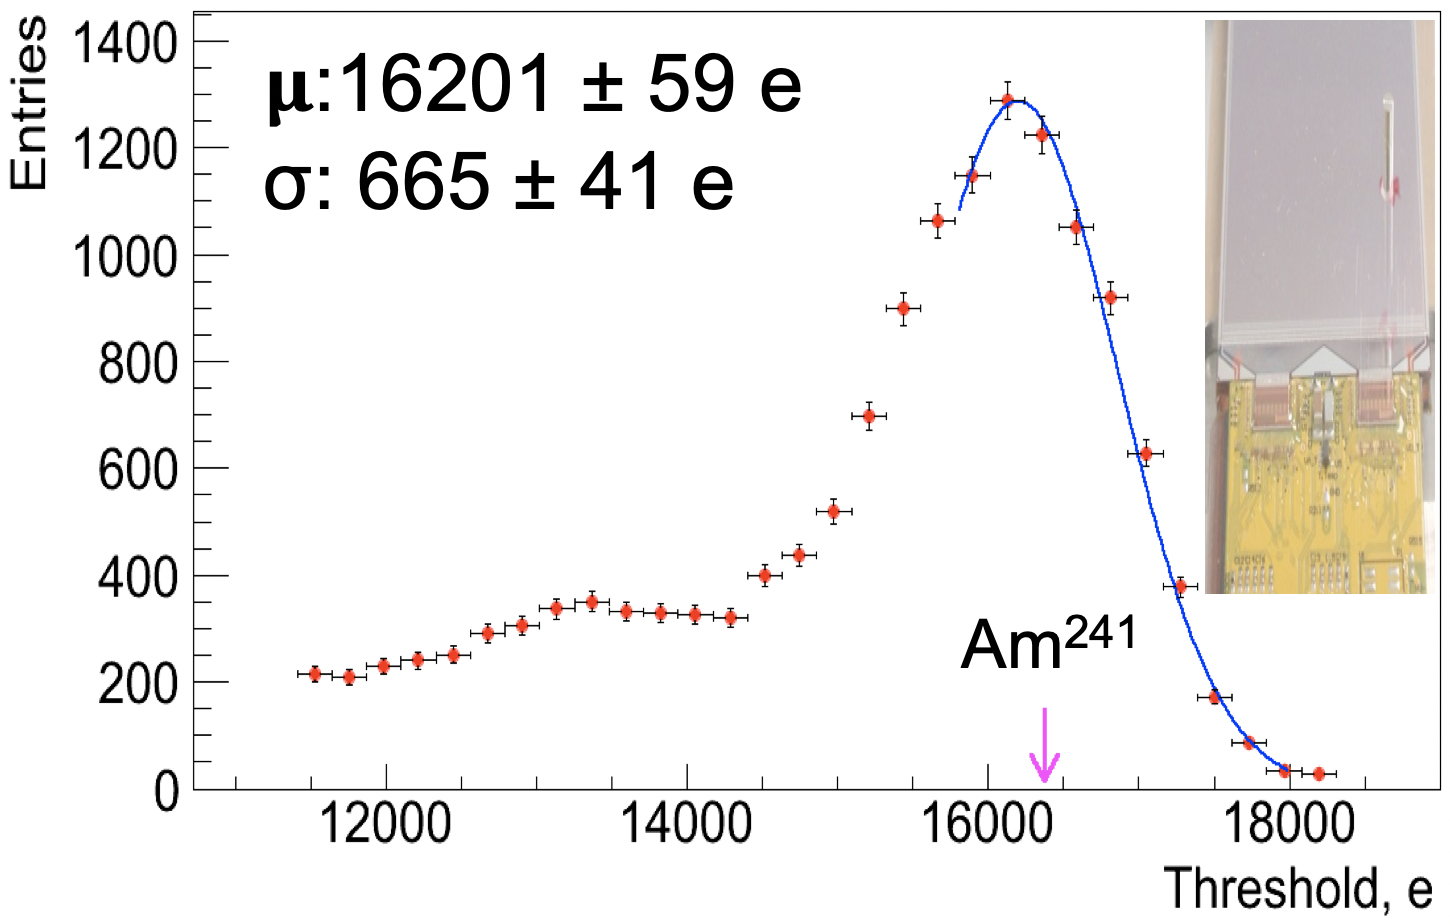
\includegraphics[width=0.5\columnwidth,keepaspectratio]{signal-gamma.png}
	\caption{Signal from Am$^{241}$ $\gamma$ source.}
	\label{fig:signal-gamma}
\end{figure}

Detector response and full readout chain calibration was done with $\gamma$ and $\beta$ sources, cosmic muons and using the proton beam. Results of absolute gain calibration with $\gamma$ source are shown in Fig.~\ref{fig:signal-gamma}. Signal peak is in good agreement with expected position. Detector response to Minimum Ionizing Particles was about 24000 electrons which is what is expected for the 320 $\mu$m thick sensor.
%
%\begin{wrapfigure}{l}{0.5\columnwidth}
%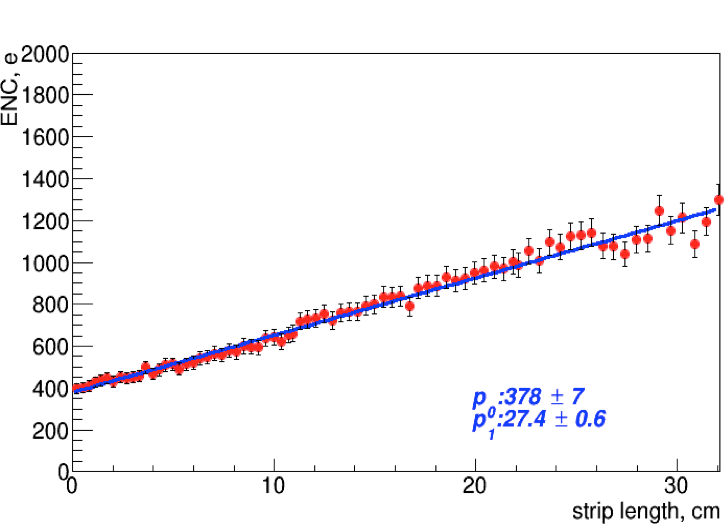
\includegraphics[width=0.5\columnwidth]{encstriplength.png}
%\caption{Input noise vs. strip length.}
%\label{fig:encstriplength}
%\end{wrapfigure}
%Longer silicon strips have higher capacitance and thus a higher expected value for the input noise. 
%(see Fig.~\ref{fig:encstriplength}).
%

%\begin{wrapfigure}{l}{0.5\columnwidth}
%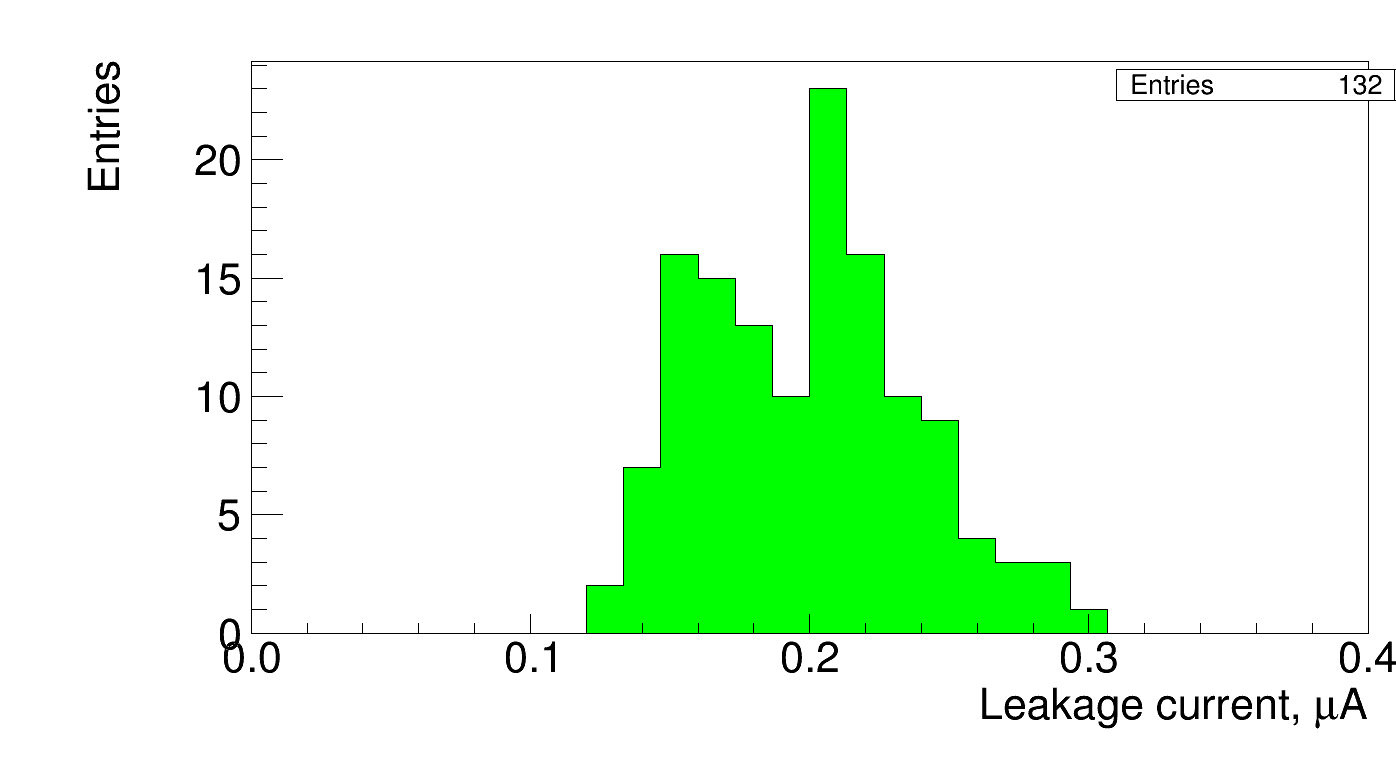
\includegraphics[width=0.5\columnwidth]{currents.png}
%\caption{Leakage currents}
%\label{fig:currents}
%\end{wrapfigure}
%
%\begin{wrapfigure}{l}{0.5\columnwidth}
%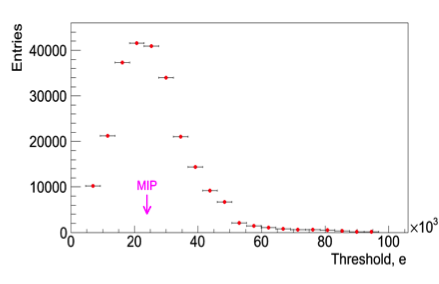
\includegraphics[width=0.5\columnwidth]{signal-muons.png}
%\caption{Signal muons}
%\label{fig:signal-muons}
%\end{wrapfigure}

